%!TEX root = ../article.tex

In this section, we present the design and the implementation of the framework, the method preliminary is also presented.
\section{Data Collection and Methodology}

\subsection{Log Collection}
The logstash which is one of the key part of ELK is used as the log collector of our framework.

\subsection{QA Knowledge data Collection}

We build a web crawler framework to collect QA knowledge data from some famous QA site like StackOverflow, in which users ask and answer questions about software development,algorithms, math and other technical topics.The users participate in activities could earn users reputation by asking and answering questions. the reputation on the site is an indicator of the value of that user contribute to the site. From this point view, the answer from a user who have a good reputation on the site could be adopted by the one asking the questions. In general,when we get a troublesome issue when diagnosing the OpenStack Platform based on the error log, we could try to troubleshoot the issue via StackOverflow directly. In order to speed up the pace of troubleshooting, we build a Knowledge repository on OpenStack.Figure 3 shows a schematic the work-flow of the crawler to collect data from QA site.In this paper, we pick StackOverflow as an example to finish the experiment. \\
\begin{figure}[!h]
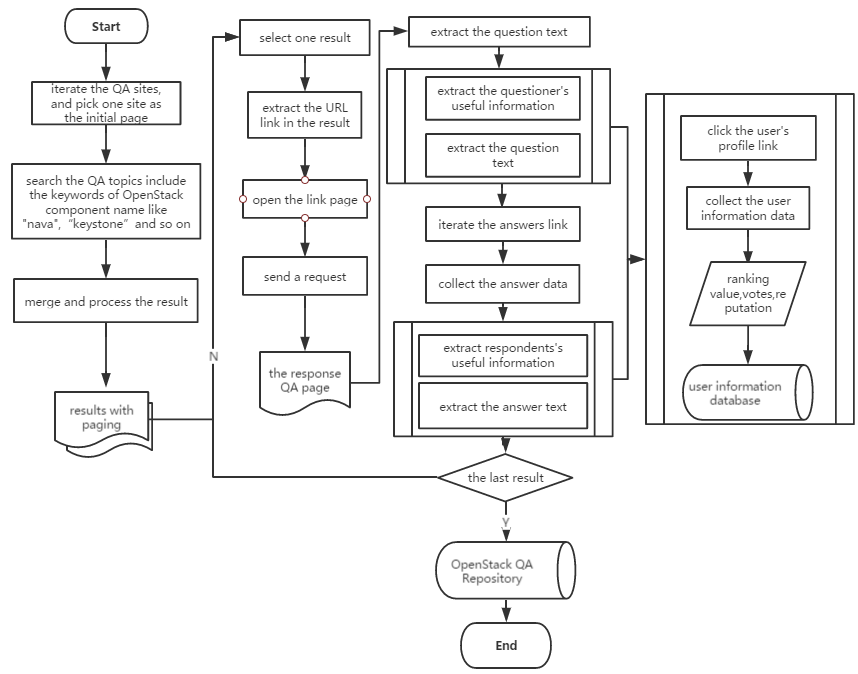
\includegraphics[scale=0.5]{./figures/Fig3.png} 
\caption{the work-flow of the crawler for collecting QA data}
\end{figure}


\renewcommand{\algorithmicrequire}{\textbf{Input:}} 
\renewcommand{\algorithmicensure}{\textbf{Output:}}

\begin{algorithm} %算法开始 
\caption{core algorithm for collecting QA data} %算法的题目 
\label{alg1} %算法的标签 
\begin{algorithmic}[1] %此处的[1]控制一下算法中的每句前面都有标号 
\REQUIRE Text:Keywords of OpenStack component,QA sites list. Variables:$list\_keywords\_openstack,list\_QA\_sites$. %输入条件(此处的REQUIRE默认关键字为Require,在上面已自定义为Input) 
\ENSURE QA information on OpenStack dataset $repo\_data$%输出结果(此处的ENSURE默认关键字为Ensure在上面已自定义为Output) 
\FOR{$site\_link$ in $list\_QA\_sites$} 

\FOR{$keyword$ in $list\_keywords\_openstack$} 
\STATE  $search\_result$ = $http\_request($$site\_link$$,$$keyword$$)$
\STATE  $search\_results.add($$search\_result$$)$
\ENDFOR

\ENDFOR

\FOR{$result$ in $search\_results$}
\STATE	$link\_topic$ = $results.link$
\STATE  {$response\_data$ = $http\_request($$link\_topic$$)$}
\STATE  {$text$ = $response\_data.question\_title$}
\STATE  $profile$ = $http\_request($$response\_data.profile\_link$$)$
\STATE  $repo\_data.add($$text$$)$
\STATE  $repo\_data.add($$profile$$)$
\STATE $answers\_results$ = $response\_data.answers$
\FOR {$answer$ in $answers\_results$}
\STATE  $answer\_text$ = $answer.content$
\STATE  $owner\_profile$ = $http\_request($$answer.owner\_link$$)$
\STATE  $repo\_data.add($$answer\_text$$)$
\STATE  $repo\_data.add($$owner\_profile$$)$
\ENDFOR
\ENDFOR
\STATE return $repo\_data$

\end{algorithmic} 
\end{algorithm}

\newcommand{\tabincell}[2]{
\begin{tabular}{@{}#1@{}}#2\end{tabular}
} 
\begin{table}[!t]  
  \centering  
  \scriptsize  
  \caption{User Schema information}  
  \begin{tabular}{ll}  
    \\[-2mm]  
    \hline  
    \hline\\[-2mm]  
    {\bf \small Key}&\qquad {\bf\small Description}\\  
    \hline  
    \vspace{1mm}\\[-3mm]  
    $id$      &   \tabincell{l}{identity of the user}\\  
    \vspace{1mm}  
    $source$          &  \tabincell{l}{source link of the source QA site}\\  
     \vspace{1mm}  
    $name$          &  \tabincell{l}{user name}\\  
     \vspace{1mm}  
    $votes$  &   \tabincell{l}{the vote count from other users from the underlying site}\\  
  	\vspace{1mm}  
    $answer\_num$  &   \tabincell{l}{the total count of answers that the user submit}\\  
     \vspace{1mm}  
    $ranking$  &   \tabincell{l}{the ranking level (percentage) in the QA site}\\  
     \vspace{1mm}  
    $top_tags$  &   \tabincell{l}{areas that the user is familiar with}\\  
     \vspace{1mm}  
    $repuataion$  &   \tabincell{l}{ reputation information}\\  
    \hline  
    \hline  
  \end{tabular}  
\end{table}  

\begin{table}[!t]  
  \centering  
  \scriptsize  
  \caption{question schema information}  
  \begin{tabular}{ll}  
    \\[-2mm]  
    \hline  
    \hline\\[-2mm]  
    {\bf \small Key}&\qquad {\bf\small Description}\\  
    \hline  
    \vspace{1mm}\\[-3mm]  
    $id$      &   \tabincell{l}{identity of the user}\\  
    \vspace{1mm}  
    $title$          &  \tabincell{l}{the title of the question}\\  
     \vspace{1mm}  
    $desc$          &  \tabincell{l}{the description/text of the question}\\  
     \vspace{1mm}  
    $votes$  &   \tabincell{l}{the vote count from other users from the underlying site}\\  
  	\vspace{1mm}  
    $tag$  &   \tabincell{l}{areas that the question belongs to}\\  
     \vspace{1mm}  
    $start\_time$  &   \tabincell{l}{the timestamp the question was created}\\  
     \vspace{1mm}   
    $update\_time$  &   \tabincell{l}{the timestamp the question was updated}\\  
      \vspace{1mm}  
    $user\_id$  &   \tabincell{l}{user id}\\  
    \hline  
    \hline  
  \end{tabular}  
\end{table} 

\begin{table}[!t]  
  \centering  
  \scriptsize  
  \caption{answer schema information}  
  \begin{tabular}{ll}  
    \\[-2mm]  
    \hline  
    \hline\\[-2mm]  
    {\bf \small Key}&\qquad {\bf\small Description}\\  
    \hline  
    \vspace{1mm}\\[-3mm]  
    $id$      &   \tabincell{l}{identity id}\\
    \vspace{1mm}  
    $user\_id$          &  \tabincell{l}{user id}\\    
    \vspace{1mm}  
    $start\_time$          &  \tabincell{l}{the timestamp the answer was created}\\  
     \vspace{1mm}  
    $update\_time$          &  \tabincell{l}{the timestamp the answer was updated}\\  
     \vspace{1mm}  
    $votes$          &  \tabincell{l}{the vote count from other users from the underlying site}\\  

    \hline  
    \hline  
  \end{tabular}  
\end{table} 


\begin{table}[!t]  
  \centering  
  \scriptsize  
  \caption{comments schema information}  
  \begin{tabular}{ll}  
    \\[-2mm]  
    \hline  
    \hline\\[-2mm]  
    {\bf \small Key}&\qquad {\bf\small Description}\\  
    \hline  
    \vspace{1mm}\\[-3mm]  
    $id$      &   \tabincell{l}{identity id}\\  
    \vspace{1mm} 
     $desc$          &  \tabincell{l}{the description/text of the answer}\\  
     \vspace{1mm}   
    $user\_id$          &  \tabincell{l}{user id}\\  
     \vspace{1mm}  
    $start\_time$          &  \tabincell{l}{the timestamp the answer was created}\\  
     \vspace{1mm}  
    $sequence$  &   \tabincell{l}{indicator of the sort order for the comments}\\  
  	\vspace{1mm}  
    $desc$  &   \tabincell{l}{the content of the comment}\\  
     \vspace{1mm}  
    $target\_type$  &   \tabincell{l}{ a label to distinguish comments for question or answer}\\  
     \vspace{1mm}  
    $target\_id$  &   \tabincell{l}{foreign key to the answer or the question}\\  
    \hline  
    \hline  
  \end{tabular}  
\end{table}

\subsection{Methodology Preliminary}
\subsubsection{Method for Data prediction}
\subsubsection{Method for Log/Topic Classification}
\subsection{Our Innovation}
In this section, we present our methodology contribution and innovation in this paper.